\documentclass[journal, a4paper]{IEEEtran}

% some very useful LaTeX packages include:

%\usepackage{cite}      % Written by Donald Arseneau
                        % V1.6 and later of IEEEtran pre-defines the format
                        % of the cite.sty package \cite{} output to follow
                        % that of IEEE. Loading the cite package will
                        % result in citation numbers being automatically
                        % sorted and properly "ranged". i.e.,
                        % [1], [9], [2], [7], [5], [6]
                        % (without using cite.sty)
                        % will become:
                        % [1], [2], [5]--[7], [9] (using cite.sty)
                        % cite.sty's \cite will automatically add leading
                        % space, if needed. Use cite.sty's noadjust option
                        % (cite.sty V3.8 and later) if you want to turn this
                        % off. cite.sty is already installed on most LaTeX
                        % systems. The latest version can be obtained at:
                        % http://www.ctan.org/tex-archive/macros/latex/contrib/supported/cite/

\usepackage{graphicx}   % Written by David Carlisle and Sebastian Rahtz
                        % Required if you want graphics, photos, etc.
                        % graphicx.sty is already installed on most LaTeX
                        % systems. The latest version and documentation can
                        % be obtained at:
                        % http://www.ctan.org/tex-archive/macros/latex/required/graphics/
                        % Another good source of documentation is "Using
                        % Imported Graphics in LaTeX2e" by Keith Reckdahl
                        % which can be found as esplatex.ps and epslatex.pdf
                        % at: http://www.ctan.org/tex-archive/info/

%\usepackage{psfrag}    % Written by Craig Barratt, Michael C. Grant,
                        % and David Carlisle
                        % This package allows you to substitute LaTeX
                        % commands for text in imported EPS graphic files.
                        % In this way, LaTeX symbols can be placed into
                        % graphics that have been generated by other
                        % applications. You must use latex->dvips->ps2pdf
                        % workflow (not direct pdf output from pdflatex) if
                        % you wish to use this capability because it works
                        % via some PostScript tricks. Alternatively, the
                        % graphics could be processed as separate files via
                        % psfrag and dvips, then converted to PDF for
                        % inclusion in the main file which uses pdflatex.
                        % Docs are in "The PSfrag System" by Michael C. Grant
                        % and David Carlisle. There is also some information
                        % about using psfrag in "Using Imported Graphics in
                        % LaTeX2e" by Keith Reckdahl which documents the
                        % graphicx package (see above). The psfrag package
                        % and documentation can be obtained at:
                        % http://www.ctan.org/tex-archive/macros/latex/contrib/supported/psfrag/

%\usepackage{subfigure} % Written by Steven Douglas Cochran
                        % This package makes it easy to put subfigures
                        % in your figures. i.e., "figure 1a and 1b"
                        % Docs are in "Using Imported Graphics in LaTeX2e"
                        % by Keith Reckdahl which also documents the graphicx
                        % package (see above). subfigure.sty is already
                        % installed on most LaTeX systems. The latest version
                        % and documentation can be obtained at:
                        % http://www.ctan.org/tex-archive/macros/latex/contrib/supported/subfigure/

\usepackage{url}        % Written by Donald Arseneau
                        % Provides better support for handling and breaking
                        % URLs. url.sty is already installed on most LaTeX
                        % systems. The latest version can be obtained at:
                        % http://www.ctan.org/tex-archive/macros/latex/contrib/other/misc/
                        % Read the url.sty source comments for usage information.

%\usepackage{stfloats}  % Written by Sigitas Tolusis
                        % Gives LaTeX2e the ability to do double column
                        % floats at the bottom of the page as well as the top.
                        % (e.g., "\begin{figure*}[!b]" is not normally
                        % possible in LaTeX2e). This is an invasive package
                        % which rewrites many portions of the LaTeX2e output
                        % routines. It may not work with other packages that
                        % modify the LaTeX2e output routine and/or with other
                        % versions of LaTeX. The latest version and
                        % documentation can be obtained at:
                        % http://www.ctan.org/tex-archive/macros/latex/contrib/supported/sttools/
                        % Documentation is contained in the stfloats.sty
                        % comments as well as in the presfull.pdf file.
                        % Do not use the stfloats baselinefloat ability as
                        % IEEE does not allow \baselineskip to stretch.
                        % Authors submitting work to the IEEE should note
                        % that IEEE rarely uses double column equations and
                        % that authors should try to avoid such use.
                        % Do not be tempted to use the cuted.sty or
                        % midfloat.sty package (by the same author) as IEEE
                        % does not format its papers in such ways.

\usepackage{amsmath}    % From the American Mathematical Society
                        % A popular package that provides many helpful commands
                        % for dealing with mathematics. Note that the AMSmath
                        % package sets \interdisplaylinepenalty to 10000 thus
                        % preventing page breaks from occurring within multiline
                        % equations. Use:
%\interdisplaylinepenalty=2500
                        % after loading amsmath to restore such page breaks
                        % as IEEEtran.cls normally does. amsmath.sty is already
                        % installed on most LaTeX systems. The latest version
                        % and documentation can be obtained at:
                        % http://www.ctan.org/tex-archive/macros/latex/required/amslatex/math/



% Other popular packages for formatting tables and equations include:

%\usepackage{array}
% Frank Mittelbach's and David Carlisle's array.sty which improves the
% LaTeX2e array and tabular environments to provide better appearances and
% additional user controls. array.sty is already installed on most systems.
% The latest version and documentation can be obtained at:
% http://www.ctan.org/tex-archive/macros/latex/required/tools/

% V1.6 of IEEEtran contains the IEEEeqnarray family of commands that can
% be used to generate multiline equations as well as matrices, tables, etc.

% Also of notable interest:
% Scott Pakin's eqparbox package for creating (automatically sized) equal
% width boxes. Available:
% http://www.ctan.org/tex-archive/macros/latex/contrib/supported/eqparbox/

% *** Do not adjust lengths that control margins, column widths, etc. ***
% *** Do not use packages that alter fonts (such as pslatex).         ***
% There should be no need to do such things with IEEEtran.cls V1.6 and later.


% Your document starts here!
\begin{document}
\begin{titlepage}

\newcommand{\HRule}{\rule{\linewidth}{0.5mm}} % Defines a new command for the horizontal lines, change thickness here

\center % Center everything on the page
 %----------------------------------------------------------------------------------------
%	LOGO SECTION
%----------------------------------------------------------------------------------------

~\\[1cm]

\includegraphics{SCUT.png}\\[2cm] % Include a department/university logo - this will require the graphicx package

%----------------------------------------------------------------------------------------
%	TITLE SECTION
%----------------------------------------------------------------------------------------

\HRule \\[1cm]
{ \huge \bfseries The Experiment Report of \textit{Machine Learning} }\\[0.6cm] % Title of your document
\HRule \\[2cm]
%----------------------------------------------------------------------------------------
%	HEADING SECTIONS
%----------------------------------------------------------------------------------------


\textsc{\LARGE \textbf{School:} School of Software Engineering}\\[1cm]
\textsc{\LARGE \textbf{Subject:} Software Engineering}\\[2cm] 

 
%----------------------------------------------------------------------------------------
%	AUTHOR SECTION
%----------------------------------------------------------------------------------------

\begin{minipage}{0.4\textwidth}
\begin{flushleft} \large
\emph{Author:}\\
Biquan Wang % Your name
\end{flushleft}
\end{minipage}
~
\begin{minipage}{0.4\textwidth}
\begin{flushright} \large
\emph{Supervisor:} \\
Qingyao Wu % Supervisor's Name
\end{flushright}
\end{minipage}\\[2cm]
~
\begin{minipage}{0.4\textwidth}
\begin{flushleft} \large
\emph{Student ID:}\\
201821038853
\end{flushleft}
\end{minipage}
~
\begin{minipage}{0.4\textwidth}
\begin{flushright} \large
\emph{Grade:} \\
Graduate
\end{flushright}
\end{minipage}\\[2cm]

% If you don't want a supervisor, uncomment the two lines below and remove the section above
%\Large \emph{Author:}\\
%John \textsc{Smith}\\[3cm] % Your name

%----------------------------------------------------------------------------------------
%	DATE SECTION
%----------------------------------------------------------------------------------------

{\large \today}\\[2cm] % Date, change the \today to a set date if you want to be precise

 
%----------------------------------------------------------------------------------------

\vfill % Fill the rest of the page with whitespace

\end{titlepage}

% Define document title and author
	\title{Logistic Regression and Support Vector Machine}
	\maketitle

% Write abstract here
\begin{abstract}
Logistic regression and Support Vector Machine are simple and efficient classification models,both of them are widely used in production. In this report, we try to compare the result with different learn rate and find out the best.
\end{abstract}

% Each section begins with a \section{title} command
\section{Introduction}
	% \PARstart{}{} creates a tall first letter for this first paragraph
\PARstart{L}{ogistic} regression is a classification model in machine learning. Due to its simplicity and efficiency, it is widely used in production.
Svm (Support Vector Machine) is a linear classifier, proposed by Cortes and Vapnik in 1995, and has been applied in the fields of handwriting recognition and text categorization, etc. This paper focuses on the mathematical model and parameter solving method of logistic regression algorithm and support vector machine algorithm. Futher more, we shows the implemention of tthese two algorithm and the result of them.
% Main Part
\section{Methods and Theory}
In this section, we will give a complete introduction to these experiments including the loss function and  the method of updating parameter $\boldsymbol{w}$ of logistic regression,  the loss function and  the method of updating parameter $\boldsymbol{w}$ of linear classification.

\subsection{Theory of logistic regression}
Assume that the labels are binary: $y_i\in\{0,1\}$
\begin{displaymath}
h_{\boldsymbol{w}}(\boldsymbol{x})=g(\boldsymbol{w}^T\boldsymbol{x})=\frac{1}{1+e^{-\boldsymbol{w}^T\boldsymbol{x}}}
\end{displaymath}
Probability:
\begin{displaymath}
p = \left\{ \begin{array}{ll}
h_w(x_i) & \textrm{$y_i=1$}\\
1-h_w(x_i) & \textrm{$y_i=0$}
\end{array} \right.
\end{displaymath}

\begin{eqnarray}
\lefteqn{ max\prod_{i=1}^nP(y_i|\boldsymbol{x_i})\Leftrightarrow max \:log(\prod_{i=1}^nP(y_i|\boldsymbol{x_i})) }
\nonumber\\
& & {}\equiv max \sum_{i=1}^nlogP(y_i|\boldsymbol{x_i})
\nonumber\\
& & {}\Leftrightarrow min -\frac{1}{n}\sum_{i=1}^nlogP(y_i|\boldsymbol{x_i})
\end{eqnarray}

\begin{displaymath}
P(y_i|\boldsymbol{x_i})=h_{\boldsymbol{w}}(\boldsymbol{x_i})^{y_i}\cdot (1-h_{\boldsymbol{w}}(\boldsymbol{x_i}))^{(1-y_i)}
\end{displaymath}
We can get the loss function:
\begin{eqnarray}
J(\boldsymbol{w})=-\frac{1}{n}\biggl[\sum_{i=1}^ny_i log h_{\boldsymbol{x}_i}+(1-y_i)log(1-h_{\boldsymbol{w}}(\boldsymbol{x}_i))\biggr]
\end{eqnarray}
The gradient of the loss function:
\begin{eqnarray}
\frac{\partial J(\boldsymbol{w})}{\partial \boldsymbol{w}}=\frac{1}{n}\sum_{i=1}^n(h_{\boldsymbol{w}}(\boldsymbol{x}_i)-y)\boldsymbol{x}_i
\end{eqnarray}
So, the update function of $w$ is:
\begin{eqnarray}
\boldsymbol{w}:=\boldsymbol{w}-\frac{1}{n}\sum_{i=1}^n(h_{\boldsymbol{w}}(\boldsymbol{x}_i)-y)\boldsymbol{x}_i
\end{eqnarray}

\subsection{Theory of linear regression}
Select two parallel hyperplanes that separate the two classes of data and let the distance between them as large as possible, The region bounded by these two hyperplanes is called the
\textbf{"margin"}.

\begin{displaymath}
L_i=\sum_{j\not=y_i}max(f_j-f_{y_i}+\Delta)
\end{displaymath}
\begin{displaymath}
f=w*x
\end{displaymath}
So:
\begin{displaymath}
L_i=\sum_{j\not=y_i}max(w^T_jx_i-w^T_{y_i}x_i+\Delta)
\end{displaymath}
Average on the train set:
\begin{displaymath}
L=\frac{1}{N}\sum_{i=1}^N\sum_{j\not=y_i}max(0,w^T_jx_i-w^T_{y_i}x_i+\Delta)
\end{displaymath}
Contain regularization:
\begin{eqnarray}
L & = & \frac{1}{N}\sum_{i=1}^N\sum_{j\not=y_i}max(0,w^T_jx_i-w^T_{y_i}x_i+\Delta){}
\nonumber\\
& & {}+ \lambda \sum_k\sum_l W_{k,l}^2
\end{eqnarray}
Gradient/derivative:
\begin{eqnarray}
\frac{\partial L_i}{\partial w_{y_i}}=-(\sum_{j\not=y_i}1(w_j^Tx_i - w_{y_i}^T x_i+\Delta >0))x_i+2\lambda w_{y_i}
\end{eqnarray}
\begin{eqnarray}
\frac{\partial L_i}{\partial w_{j}}=1(w_j^Tx_i-w_{y_i}^Tx_i+\delta>0)x_i+2\lambda w_j
\end{eqnarray}

\section{Experiments}
\subsection{Dataset}
Experiment uses a9a of LIBSVM Data, including 32561/16281(testing) samples and each sample has 123/123 (testing) features.

\subsection{Step of Logistic regression}
The steps of our Logistic regression are as the following:
\begin{itemize}
\item[1.] Use load\_svmlight\_file function in sklearn library to load the a9a as train set a9a.t as valid set.
\item[2.] change the value of $y$ from (1,-1) to (1,0).
\item[3.]Initialize logistic regression model parameters. Set all parameter into zero, initialize it randomly or with normal distribution.
\item[4.] Get a mini-batch data from train set randomly.
\item[5.] Update the parameters $\boldsymbol{w}$ with function (4)
\item[6.] Calculate the loss of train set and validation set with function (2).
\item[7.] Calculate the threshold loss of validation set, mark the sample whose predict scores greater than the threshold as positive, on the contrary as negative.
\item[8.] Repeate setp 4-7 for n times, and return the losses of train set, losses of validation set and the threshold losses.
\end{itemize}

\subsection{Result of Logistic regression}
In logistic regression, we discuss the impact with different value of learning rate, other prameter is same: interaction:1000,threshold:0.5, and batch size:64. By visualized as a figure, we try to get a proper value of learning rate and analyze the causes of different results. 
\begin{figure}[!htb]
	\begin{center}
	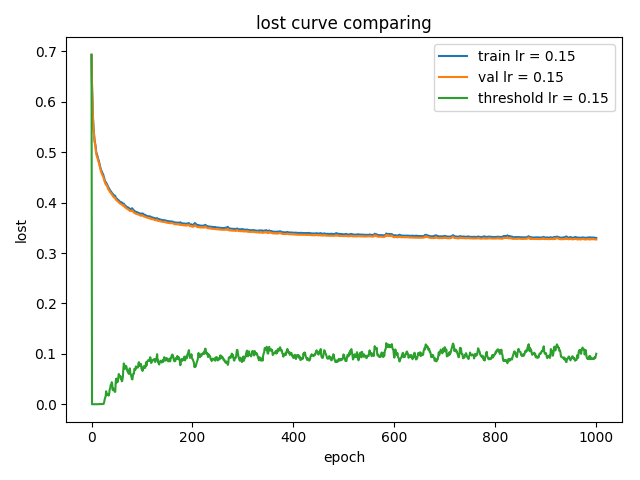
\includegraphics[width=\columnwidth]{logr_15}
	\caption{Logistic regression learn rate:0.15}
	\label{fig:logr_15}
	\end{center}
\end{figure}

\begin{figure}[!htb]
	\begin{center}
	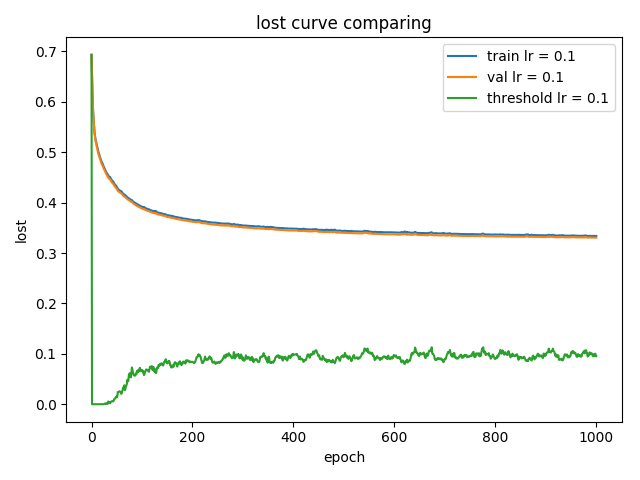
\includegraphics[width=\columnwidth]{logr_10}
	\caption{Logistic regression learn rate:0.1}
	\label{fig:logr_10}
	\end{center}
\end{figure}

\begin{figure}[!htb]
	\begin{center}
	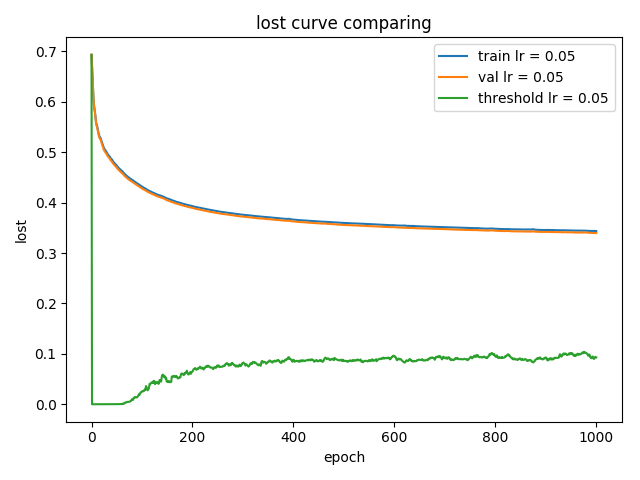
\includegraphics[width=\columnwidth]{logr_05}
	\caption{Logistic regression learn rate:0.05}
	\label{fig:logr_05}
	\end{center}
\end{figure}
\begin{figure}[!htb]
	\begin{center}
	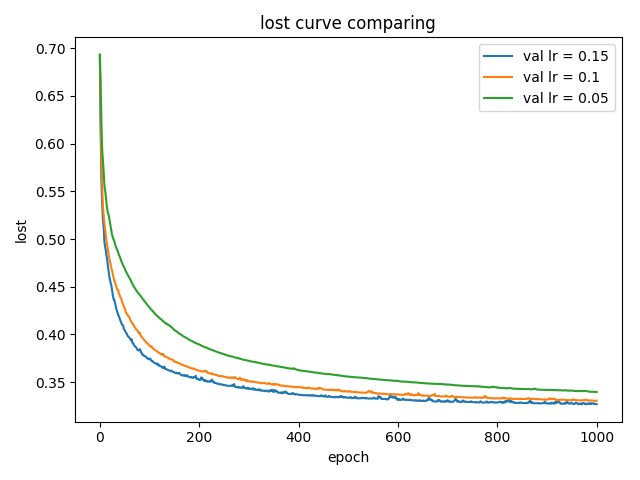
\includegraphics[width=\columnwidth]{logr_val_cp}
	\caption{Valid loss compare of different learn rate}
	\label{fig:logr_val_cp}
	\end{center}
\end{figure}

In figure 1 2 3 4, we can find out that during the learning rate increasing, the validation loss decrease progressively. However, when the learning rate is out of a boundary, the loss will be vibrating and can not achieve the best performance.

\subsection{Step of SVM}
The steps of our SVM are as the following:
\begin{itemize}
\item[1.] Use load\_svmlight\_file function in sklearn library to load the a9a as train set a9a.t as valid set.
\item[2.] change the value of $y$ from (1,-1) to (1,0).
\item[3.]Initialize SVM model parameters. Set all parameter into zero, initialize it randomly or with normal distribution.
\item[4.] Get a mini-batch data from train set randomly.
\item[5.] Update the parameters $\boldsymbol{w}$ with function (6) and (7)
\item[6.] Calculate the loss of train set and validation set with function (5).
\item[7.] Calculate the threshold loss of validation set, mark the sample whose predict scores greater than the threshold as positive, on the contrary as negative.
\item[8.] Repeate setp 4-7 for n times, and return the losses of train set, losses of validation set and the threshold losses.
\end{itemize}

\subsection{Result of SVM}
In SVM, we try to compare the different loss with different learning rate, other prameter is same: interaction:500,regular:0.5, and batch size:64.

\begin{figure}[!htb]
	\begin{center}
	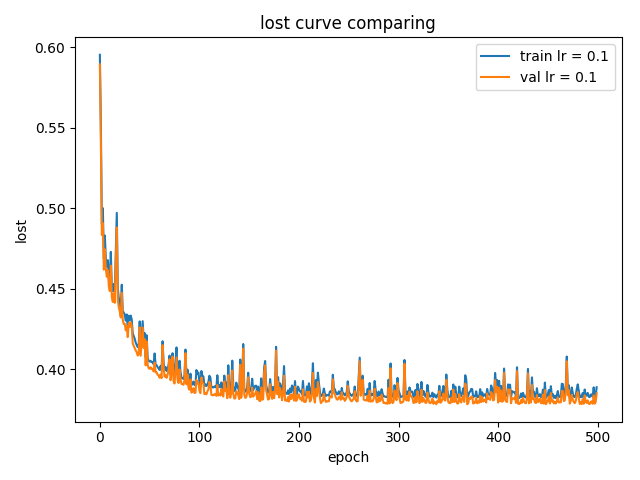
\includegraphics[width=\columnwidth]{lc_1}
	\caption{SVM learn rate:0.1}
	\label{fig:lc_1}
	\end{center}
\end{figure}

\begin{figure}[!htb]
	\begin{center}
	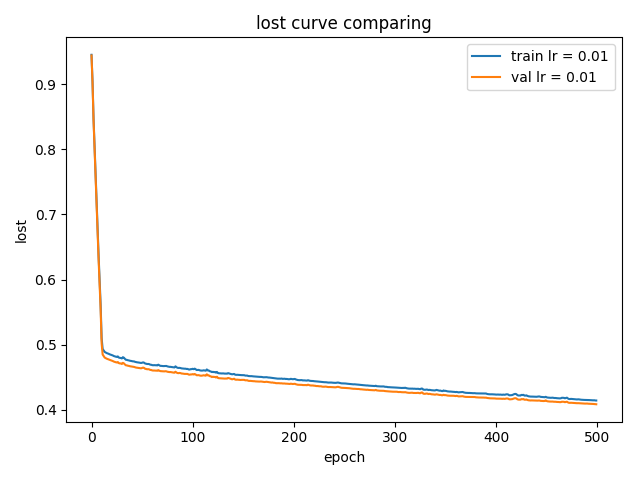
\includegraphics[width=\columnwidth]{lc_01}
	\caption{SVM learn rate:0.01}
	\label{fig:lc_01}
	\end{center}
\end{figure}

\begin{figure}[!htb]
	\begin{center}
	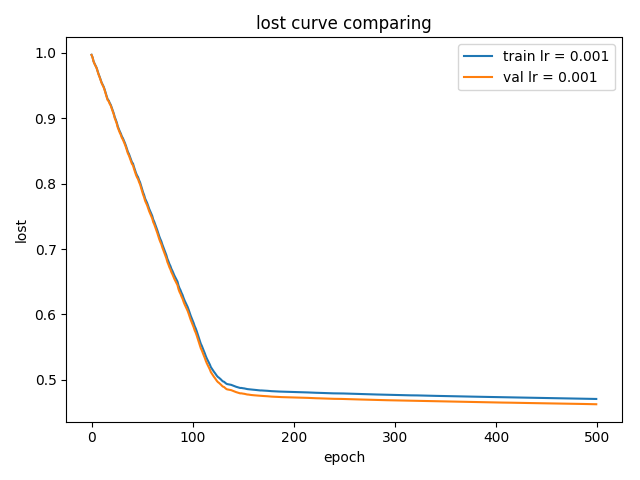
\includegraphics[width=\columnwidth]{lc_001}
	\caption{SVM learn rate:0.001}
	\label{fig:lc_001}
	\end{center}
\end{figure}
\begin{figure}[!htb]
	\begin{center}
	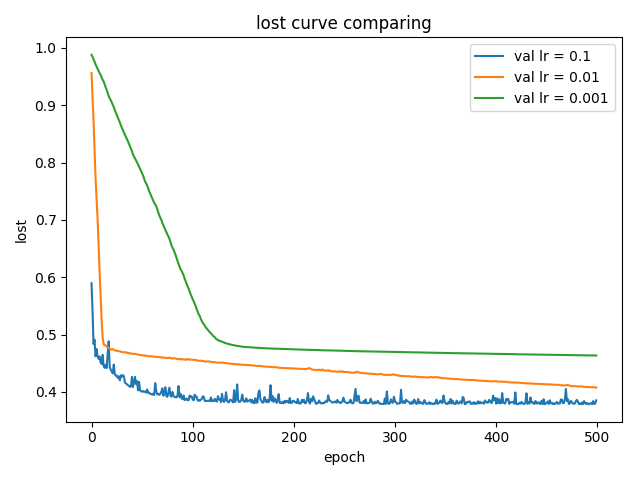
\includegraphics[width=\columnwidth]{lc_val_cp}
	\caption{SVM Valid loss compare of different learn rate}
	\label{fig:lc_val_cp}
	\end{center}
\end{figure}
\section{Conclusion}
In this reprot, we mentioned Logistic regression and Support Vector Machine, both of them use  SGD to approach the solution. For esaier to understand, we try to conduct some experiments and visualize the results of logistic regression and SVM and try to compare and analys the result. 

% Your document ends here!
\end{document}